%----------------------------------------------------------------------------------------
%	PACKAGES AND DOCUMENT CONFIGURATIONS
%----------------------------------------------------------------------------------------
\documentclass{article}

\usepackage{graphicx} 	% Required for the inclusion of images
\usepackage{natbib} 	% Required to change bibliography style to APA
\usepackage{amsmath} 	% Required for some math elements 
\usepackage{array}
\usepackage{caption}
\usepackage{subcaption}

\usepackage{xcolor}
\usepackage{listings}
\usepackage{color}		 %red, green, blue, yellow, cyan, magenta, black, white
\usepackage{geometry}
\geometry{
a4paper,
total={170mm,257mm},
left=20mm,
top=20mm,
}
\setlength\parindent{0pt} % Removes all indentation from paragraphs

\definecolor{codegreen}{rgb}{0,0.6,0}
\definecolor{codegray}{rgb}{0.5,0.5,0.5}
\definecolor{codepurple}{rgb}{0.58,0,0.82}
\definecolor{backcolour}{rgb}{0.9,0.9,0.9}

\lstdefinestyle{mystyle}{
    %backgroundcolor=\color{backcolour},   
    frame=tb, 				% draw a frame at the top and bottom of the code block
    commentstyle=\color{codegreen},
    keywordstyle=\color{magenta},
    numberstyle=\tiny\color{codegray},
    stringstyle=\color{codepurple},
    basicstyle=\footnotesize,
    breakatwhitespace=false,         
    breaklines=true,                 
    captionpos=b,                    
    keepspaces=true,                 
    numbers=left,                    
    numbersep=5pt,                  
    showspaces=false,                
    showstringspaces=false,
    showtabs=false,                  
    tabsize=4
}
\lstset{style=mystyle}


%----------------------------------------------------------------------------------------
%	DOCUMENT INFORMATION
%----------------------------------------------------------------------------------------
\title{Artificial Intelligence in Control Engineering exercise}
\author{
	Lecturer: Dr.Pham Viet Cuong	\\
}
\date{October 08th, 2018}

\begin{document}
\maketitle 					% Insert the title, author and date

\begin{center}
	\begin{tabular}{l l}
	Group 9: \\
	Nguyen Chinh Thuy 	& 1513372	\\
	Nguyen Tan Phu		& 1512489	\\
	Le Van Hoang Phuong	& 1512579	\\
	Do Tieu Thien		& 1513172			\\
	Nguyen Tan Sy		& 1512872	\\
	Nguyen Van Qui		& 1512702
	\end{tabular}
\end{center}


%----------------------------------------------------------------------------------------
%	SECTION 1
%----------------------------------------------------------------------------------------
\section{Problem}

%----------------------------------------------------------------------------------------
%	SECTION 2
%----------------------------------------------------------------------------------------
\section{Configuration}

%----------------------------------------------------------------------------------------
%	SECTION 3
%----------------------------------------------------------------------------------------
\section{Implementation}
\subsection{Particle Filter}
To solve the Paticle Filter problem, we implement follow below steps: \\
\begin{itemize}
	\item{Prediction} 
	\begin{itemize}
		\item{Implementing a loop with $M$ step which is numbers of particles}
		\item{Using process model and control signals $u_t$ in \textbf{VG} which are affected by thermal noise to calculate coordinate $x^{[m]}_t$ of robot.}
		\item{Combining coordinate of robot from above step and coordinate of landmarks in \textbf{lm} to calculate range $r_t$ and bearing angle $b_t$.}
		\item{Calculating importance factor $w^{[m]}_t$ depend on probability density function fomula with $\mu$ is matrix of expected range and bearing which are from \textbf{XODO}}
		\begin{align}
			f_x(x_1,x_2,...,x_N) = \dfrac{1}{\left(2\pi\right)^{\dfrac{N}{2}}\Vert\Sigma\Vert^{\dfrac{1}{2}}}exp\left(\dfrac{-1}{2}\left(x-\mu\right)^T\Sigma^{-1}\left(x-\mu\right)\right)
		\end{align}
	\end{itemize}
	\item{Selection}
	\begin{itemize}
		\item{Implementing a loop with $M$ step.}
		\item{Choosing a index in range $\left[1,M\right]$ for $x^{[m]}_t$ with probabilities $w^{[m]}_t$.}
	\end{itemize}
\end{itemize}
\subsubsection{Python code}
\lstinputlisting[language=Python]
{../main.py}

%----------------------------------------------------------------------------------------
%	SECTION 4
%----------------------------------------------------------------------------------------
\subsubsection{Result} 
\begin{figure}[h]
\centering
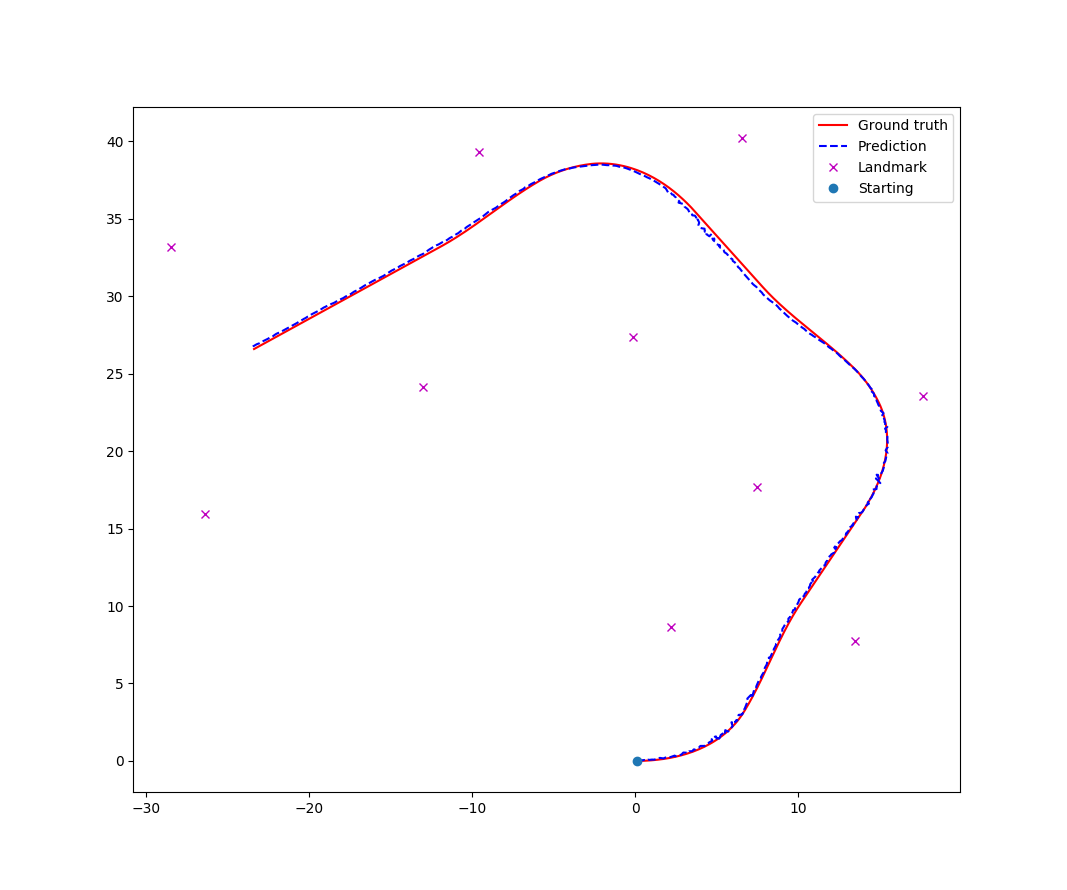
\includegraphics[width=\textwidth]{../particle-max.png}
\caption{Trajectory}\label{fig:image-1}
\end{figure}
\end{document}

